\documentclass[a4paper]{article}
\usepackage[margin=1in]{geometry} 
% \usepackage{ctex}
\usepackage{tabularx}
\usepackage{lipsum}
\usepackage{enumerate}
\usepackage{amsfonts}
\usepackage{multirow}
\usepackage{graphicx}
\usepackage{siunitx}
%\usepackage{fbox}
%\usepackage{framed}
\usepackage{tcolorbox}

\begin{document}
\begin{titlepage}
    \title{\textbf{Lab Report 4: Investigating how the volume of a fixed amount of gas affect its pressure\footnote{Consistant temperature and other controlled variables should be mentioned in variables part, which is not required in this assignment.}}}
    \author{Eric Zhou}
    \date{\today}
    \maketitle
    %\tableofcontents
\end{titlepage}

\section{Results}

Previous content is not required, and hence not included in this assignment.
\begin{figure}[h!]
    \centering
    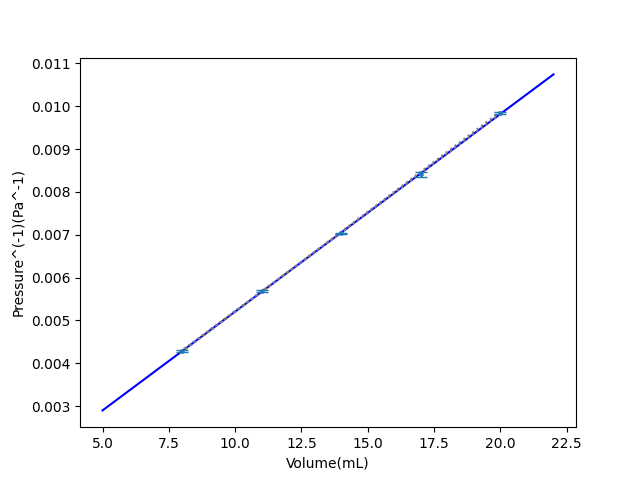
\includegraphics[width = 0.8\textwidth]{Figure_1.png}
    \caption{$p^{-1} - V$ graph}
    \label{fig}
\end{figure}

\begin{tcolorbox}[title = Note]
    Include extended graph to show x/y intercepts.
\end{tcolorbox}

\section{Discussion and conclusion}

The diagram shows a strong postive correlation of $P^{-1}$ and $V$, and its best linear fit has

\begin{itemize}
    \item A slope of $4.61518\times 10^{-4}$.
    \item A y-intercept of $5.90218\times 10^{-4}$.
\end{itemize}

As is mentioned in processed data section, the graph is expected to be a straight line passing through the origin. The diagram show a graph with relatively small error, supporting the initial hypothesis. 

The y-intercept is expected to be zero, but $5.90218\times 10^{-4}$ is found. This might have resulted from the error of barometer.

The gradient is expected to be $1\over nRT$, where $R$ is the gas contsant $R = \SI{8.31}{J\cdot mol^{-1}\cdot K^{-1}}$, $T$ is the temperature of the gas in kelvin and $n$ is the number of moles of the gas. It can be hence estimated that the gas contains about $\SI{0.87}{mmol}$ of molecules, which is a reasonable value.

Considering the small error, the results support our initial hypothesis. The air pressure decreases as the volume expands and is inversely proportional to its volume, provided the amount of the gas and the temperature remains the same. 

\begin{tcolorbox}[title = Note]
    Error bar is relatively small, indicating high precision and low random error.
    Discussion of x-intercept / y-intercept (volume in the connecting part of the syringe and the probe.) \\
    The volume can be measured using geometric method (cross section area $\times$ length, etc). \\
    Also, the effect caused by the connceting part can be reduced by switching to a larger syringe. Note that we need to balance the error reducing effect and the low accuracy. \\
    find $n$: $k = {1\over{nRT}} \Rightarrow n = {RT \over k} \Rightarrow n\approx 0.87\SI{}{mmol}$
\end{tcolorbox}

\section{Evaluation}

The experiment has been conducted successfully, gathering sufficient data and support our hypothesis. However, there is still room for imporvement.

\begin{itemize}
  \item \textbf{Temperature control:} The experiment is conducted in a short period of time, which means the heat produced due to compression and friction may not have been conducted to the surroundings. This may fail to keep the temperature, which is a vital variable that needs to be controlled, constant throughout the experiment. To improve this, we may repeat the experiment by leave the syringe in the air for a longer time to ensure sufficient heat exchange or do the experiment in constant temperature water tank.
  \item \textbf{Flaw of ideal gas model:} The model tested by the experiment is actually flawed when the temperature is not suitable or the pressure is high. To avoid that flaw, one can avoid squeeze the syringe too much and choose gas with low boiling points. However, this flaw in the model can not be ignored. It is also good to do exactly the opposite (i.e. conduct the experiment with high melting point gas and in high pressure) to investigate the flaw in the future as well.
  \item \textbf{Leak of air:} The syringe and equipment we used is not exactly air-tight and therefore a leak is very likely to happen, which is problematic because this result in change in the amount of substance $n$, another vital variable that should have been kept constant. To minimize that effect, we may choose a better equipment and avoid pushing the syringe too hard, which may accelerate the leaking.
  \item \textbf{Muscle problems:} Human muscle is subject to uncontrolable tremor when exerting force \footnote{Christakos, C. N., Papadimitriou, N. A., \& Erimaki, S. (2006). Parallel neuronal mechanisms underlying physiological force tremor in steady muscle contractions of humans. Journal of neurophysiology, 95(1), 53-66.}. To put in other words, it is hard to have the volume fixed due to the limitation of human muscle, leading to error in the readings. Use a clamp and a small wood block to keep pressing the syringe while taking down the readings can avoid this issue. 
\end{itemize}

\begin{tcolorbox}[title = Note]
    parallax error : 								more trials \\
    low precision in readings of volume in syringe \\
    fluctuation in temperature : 					compress slowly, water tank \\
    change in number of moles in each trial :			do not disconnect in each trial \\
    leak of air : 									seal, use leak detecting device \\
    not ideal gas : 								low pressure, pull rather  than squeeze \\
    vary of volume when pushing manually : 			clamp to compress \\
    check zero error of pressure probe 
\end{tcolorbox}


\end{document}